\newpage
{\bfseries МРНТИ 61.51.15}

{\bfseries STUDY OF THE EFFECTIVENESS OF THE DEMULSIFIER COMPOSITION ON THE
DESTRUCTION OF LOCAL OIL-WATER EMULSION}

{\bfseries L.K Tastanova, A.K.Apendina, R.O Orynbasar, N.Zh.Zhanserikov,
S.A. Nurlybay}

Aktobe Regional University named after K.Zhubanova, Aktobe, Kazakhstan

Corresponding author: su1tan@bk.ru

The effect of the demulsifier composition on the destruction of local
oil-water emulsions was studied in this work. One of the urgent problems
in the development of deposits is to increase the efficiency of the
preparation of hydrocarbons in the fields. The solution of this problem
makes it possible to significantly increase the degree of oil
preparation, reduce the loss of hydrocarbons with drainage waters,
thereby improve the environment and bring additional profit to the
enterprise. A complex of theoretical and experimental studies was used,
consisting in generalization and analysis of literary data, as well as
by analogy, modeling, quantitative and qualitative observation,
laboratory tests, conducting a multifactorial experiment, data
processing using methods of mathematical statistics. Information
processing tools based on computer software products were used. The
results of laboratory tests of oil-water emulsion, physico-chemical
analysis of water composition, new chemical reagents-demulsifiers
recommended for field testing are presented. It can be concluded, based
on the research conducted, that the demulsifier EASY-DE03-15 is the most
effective reagent for dehydration of oil-water emulsions and
desalination of MIX samples.

{\bfseries Keywords:} oil, demulsifier, oil-water, emulsions, efficiency,
deposit, reagent, chemistry.

{\bfseries ИССЛЕДОВАНИЕ ВЛИЯНИЯ СОСТАВА ДЕЭМУЛЬГАТОРА НА РАЗРУШЕНИЕ МЕСТНЫХ
ВОДОНЕФТЯНЫХ ЭМУЛЬСИЙ}

{\bfseries Л.К.Тастанова, А.К.Апендина, Р.О.Орынбасар,
Н.Ж.Жансериков,С.А.Нурлыбай}

Актюбинский Региональный университет имени К. Жубанова, Актобе,
Казахстан,

е-mail: su1tan@bk.ru

В работе изучена эффективность состава деэмульгатора на разрушение
местных водонефтяных эмульсии. Одной из актуальных проблем при
разработке месторождений является повышение эффективности подготовки
углеводородов на месторождениях. Решение этой задачи позволяет
значительно повысить степень подготовки нефти, снизить потери
углеводородов с дренажными водами, тем самым улучшить экологию и
принести дополнительную прибыль предприятию. Для решения поставленных
задач использовался комплекс теоретико-экспериментальных исследований,
заключающийся в обобщении и анализе литературных данных, а также по
аналогии, моделировании, количественном и качественном наблюдении,
лабораторных испытаниях, проведении многофакторного эксперимента,
обработка данных с использованием методов математической статистики.
Использовались средства обработки информации на базе компьютерных
программных продуктов. Приведены результаты лабораторных испытаний
водонефтяной эмульсии, физико-химического анализа состава воды, новых
химических реагентов-деэмульгаторов, рекомендованных для полевых
испытаний. На основе проведенного исследования установлено, что
деэмульгатор EASY-DE03-15 является наиболее эффективным реагентом по
обезвоживанию водонефтяных эмульсий и обессоливания MIX пробы.

{\bfseries Ключевые слова:} нефть, деэмульгатор, водонефтяные, эмульсия,
эффективность, месторождение, реагент, химия.

{\bfseries ЖЕРГІЛІКТІ СУ-МҰНАЙ ЭМУЛЬСИЯЛАРЫН БҰЗУҒА АРНАЛҒАН ДЕЭМУЛЬГАТОР
ҚҰРАМЫНЫҢ ТИІМДІЛІГІН ЗЕРТТЕУ}

{\bfseries Л.К.Тастанова, А.К.Апендина, Р.О.Орынбасар, Н.Ж.Жансериков,
С.Ә}.{\bfseries Нұрлыбай}

Қ. Жұбанов атындағы Ақтөбе Өңірлік университеті, Ақтөбе, Қазақстан,

е-mail: su1tan@bk.ru

Жұмыста жергілікті су-мұнай эмульсияларын жою үшін деэмульгатор
құрамының тиімділігі қарастырылды. Кен орындарын игерудегі өзекті
мәселелердің бірі кен орындарында көмірсутектерді дайындау тиімділігін
арттыру болып табылады. Бұл мәселені шешу мұнайдың дайындалу дәрежесін
едәуір арттыруға, дренажды сулармен көмірсутектердің жоғалуын азайтуға,
сол арқылы экологияны жақсартуға және кәсіпорынға қосымша пайда әкелуге
мүмкіндік береді. Қойылған міндеттерді шешу үшін әдеби деректерді
жалпылау мен талдаудан, сондай-ақ ұқсастық, модельдеу, сандық және
сапалық бақылау, зертханалық сынақтар, көп факторлы эксперимент жүргізу,
математикалық статистика әдістерін қолдана отырып өңдеу деректерінен
тұратын теориялық және эксперименттік зерттеулер кешені пайдаланылды.
Компьютерлік бағдарламалық өнімдер негізінде ақпаратты өңдеу құралдары
пайдаланылды. Су-мұнай эмульсиясының зертханалық сынақтарының
нәтижелері, су құрамының физика-химиялық талдауы, далалық сынақтарға
ұсынылған жаңа химиялық реагенттер-деэмульгаторлар келтірілген.
Зертханалық зерттеулердің нәтижелерін талдай отырып, EASY-DE03-15
деэмульгаторының су-мұнай эмульсияларын сусыздандыру және Mix сынамасын
тұзсыздандыру бойынша ең тиімді реагент екендігі анықталды.

{\bfseries Түйінді сөздер:} мұнай, деэмульгатор, су-мұнай, эмульсиялар,
тиімділік, кен орны, реагент, химия.

{\bfseries Introduction.} Currently, the formation of water-oil stable
emulsions is observed in most oil fields of Kazakhstan, the destruction
of which requires significant material and time costs. Expensive
Western-made demulsifiers are mainly used to prepare commercial oil at
all fields. There are many factors that stimulate the separation of
water from oil, but in practice none of them allows for sufficiently
deep dehydration without the use of a demulsifier. As the field is
developed, the process of "aging" of the emulsion changes, the oil-water
fraction increases, the ratio of the phase interface and the number of
natural stabilizers change. Under these conditions, the choice of a new
effective demulsifier is quite important. The spectrum of chemical
compounds used as components of demulsifying compositions is quite wide.
Foreign manufacturers have in their arsenal up to several dozen
compounds of each class, differing in molecular weight, relative
solubility, etc.{[}1{]}.

Today, fundamentally different technological schemes of oil collection
and processing operate at the fields, the conditions for processing
emulsions and their results differ significantly from object to object,
although practically the same emulsion is processed. The variety of
technological schemes and equipment used in this case has led to the
fact that demulsifiers are selected separately for each object.

Most chemical companies are well trained and equip their representatives
with the selection of demulsifiers and bringing the installation to
optimal performance. The owners of oil fields themselves do not deal
with these issues and invite representatives of other companies to
select demulsifiers and develop recommendations for their use. Instead
of choosing from hundreds of names of demulsifiers suitable for use only
in a specific installation with all its technological features, it is
necessary to develop an ideal technological scheme for oil treatment,
create effective dehydrogenation equipment based on it and use a
demulsifier corresponding to the type of refined oil {[}2{]}.

Currently used methods of oil extraction have led to the fact that up to
90\% of water is extracted with oil, forming stable oil-water emulsions
stabilized with natural surfactants and resins {[}3{]}. These natural
surfactants are asphaltenes, mechanical impurities, as well as heavy
paraffins. Other factors stabilizing oil-water emulsions are chloride
salts and the hydrogen pH of water in oil {[}4{]}.

Due to the high stability of these emulsions, their destruction is
possible only with the help of demulsifiers. The consumption of the
demulsifier is determined by the need to obtain commercial oil with a
water content of less than 0.2\%, with higher water content, the cost of
oil on the world market decreases, and at 1\% oil is considered
substandard. Since the cost of demulsifiers is quite high, the problem
of reducing their consumption by increasing efficiency is very relevant.
There are two ways to solve this problem {[}3{]}.

1. The first, chemical-technological, consists in the development of
methods for the synthesis of new reagents with demulsifying ability. The
level of these developments at a number of enterprises has reached quite
a satisfactory level.

2. Deeper dewatering of oil at low costs can be achieved with the help
of demulsifiers consisting of various chemical compounds, provided that
a synergistic effect is manifested between these compounds. The
development of such synergistic demulsifying compounds is the second way
to increase their effectiveness. However, the scientific basis of this
method of increasing the effectiveness of demulsifiers has not yet been
developed {[}5{]}.

It is important to emphasize that the demulsifiers themselves are
chemical surfactants obtained by complex multi-stage chemical synthesis,
which consist of several components {[}6{]}.

The insufficient level of scientific validity of the development of
demulsifiers is also evidenced by the lack of systematic studies of the
effect on the effectiveness of demulsifiers of the solvent nature of
their commercial forms, in the form in which they are supplied to
fisheries enterprises that have solutions from 30\% to 65\% in a certain
solvent. Although there is a large number of works on the influence of
the nature of the solvent on the speed of physico-chemical processes,
there is practically no data on the possible relationship between the
effectiveness of demulsifiers and the composition of their commercial
forms in the literature. Moreover, in most works with these reagents,
the type of solvent is not even indicated. Insufficient attention is
also paid to the consideration of the method of introducing a
demulsifier into the emulsion in the conditions of field oil treatment
{[}7{]}.

From the above it follows the need for fundamental research of the
principles that determine the mechanism of action and effectiveness of
demulsifiers. Only after such a study is it possible to solve the
problem of optimizing their composition and conditions of the
demulsification process. At the same time, the variety of properties of
oils, field development systems and demulsifiers puts optimization of
their use as an important task, both in terms of technological problems
and reducing the cost of reagents {[}8{]}.

Modern demulsifiers, most commonly used in the demulsification industry,
are surfactants that exhibit both hydrophilic and hydrophobic groups.
They have almost completely replaced the long-outdated ion-active
demulsifiers {[}9{]}. When the number of moles of ethylene and propylene
oxide changes, chemical compounds are obtained that are balanced in a
certain way in terms of hydrophobic and hydrophilic properties and have
a high demulsifying ability with respect to the emulsion of a particular
oil field. The polymer surfactant, when added to an oil emulsion, is
located at the interface between water and oil molecules. Hydrophilic
groups focus on water, while hydrophobic groups focus on oil. The best
polymer surfactants currently used worldwide are derivatives of
alkoxylated materials {[}10{]}.

It is known that the following basic requirements are imposed on modern
demulsifiers: they must have the maximum possible demulsifying activity,
be easily biodegradable, non-toxic, cheap and affordable; they must not
have bactericidal activity (on which the effectiveness of biological
wastewater treatment depends) and corrode metals. It is worth noting
that different groups of demulsifiers have not only a number of positive
properties, but also various disadvantages. So, some reagents provide
separation of pure water, but the emulsion decomposes not fast enough.
Other reagents contribute to the rapid destruction of the emulsion, but
the wastewater contains a lot of petroleum products {[}11{]}.

Many reagents are not effective enough to remove mechanical impurities.
Therefore, in recent decades, compositions have been developed
containing several individual compounds that exhibit a synergistic
effect in the mixture, since they can provide the necessary degree of
oil dehydration, where the efficiency of demulsifying the mixture of
components is higher than the effect of individual components. However,
until now, the main practice of developing demulsifiers on the world
market is the empirical selection of their composition for water-oil
emulsions of specific deposits {[}12{]}.

It is known that the reagents used to bring oil to marketable condition
include demulsifiers, mainly imported from abroad. This, in turn,
increases the cost of oil treatment. To date, the issues of determining
and applying an effective demulsifier, as well as determining its
alternative or reducing its consumption, remain relevant.

The purpose of the study is to determine the effect of demulsifiers
prepared using chemical reagents of the domestic EASY-DE brand for the
conditions of oil preparation of Meerbush LLP as well as to prove the
effectiveness of domestic-made demulsifier application in the oil and
water industry.

{\bfseries Methods and materials.} The methods and techniques of analysis
corresponding to the goals and specific tasks of the study were used in
the work. The article uses general scientific methods and approaches. To
solve the tasks set, a set of theoretical and experimental studies was
used, consisting of generalization and analysis of literary data,
testing conducted at the deposits of Western Kazakhstan, as well as by
analogy, modeling, quantitative and qualitative observation, laboratory
studies, multidimensional experiment, data processing by mathematical
statistics methods. In addition, methods of constructing algorithms and
flowcharts were used. Information processing tools based on computer
software products were used.

The sequence of laboratory tests is as follows:

1. Simulation of the "bottle test" with determination of laboratory
conditions (demulsifier input temperature, separation temperature and
time, amount of shaking and oil extraction level for centrifugation);

2. Determination of oil sampling points and composition of oil-water
emulsion mixture;

3. Conducting a "bottle test" of all provided reagents in comparison
with the base reagent (used in the field) in different dosages;

4. Determination of the content of chloride salts in oil SUST 215-34;

5. Analysis of the results obtained and recommendation of demulsifiers
for PIT (pilot tests) {[}13{]}.

Test progress:

The tests were conducted on March 10-15, 2022.

For testing, a sample of oil was taken on February 02 from the birth of
Kulzhan LLP "Meerbusch", Ayyrshagyl LLP "BNGltd".

An oil sample from the Ayyrshagyl site of BNGltd LLP was taken from the
well on February 02 №141, №143, №145, №150, №151, №153, №154.

The physical and chemical properties of oil used in study are presented
in Table 1.

{\bfseries Table 1 Physical and chemical properties of oil from the Kulzhan
and Ayyrshagyl fields}

\begin{longtable}[]{@{}
  >{\raggedright\arraybackslash}p{(\columnwidth - 4\tabcolsep) * \real{0.3354}}
  >{\raggedright\arraybackslash}p{(\columnwidth - 4\tabcolsep) * \real{0.3311}}
  >{\raggedright\arraybackslash}p{(\columnwidth - 4\tabcolsep) * \real{0.3335}}@{}}
\toprule\noalign{}
\begin{minipage}[b]{\linewidth}\raggedright
Characteristics
\end{minipage} & \begin{minipage}[b]{\linewidth}\raggedright
Crude oil from the Kulzhan oilfield
\end{minipage} & \begin{minipage}[b]{\linewidth}\raggedright
Crude oil from the Ayyrshagyl oilfield
\end{minipage} \\
\midrule\noalign{}
\endhead
\bottomrule\noalign{}
\endlastfoot
Density at 20\textsuperscript{0}С, g/sm\textsuperscript{3} & 0.8747 &
0.8704 \\
Water content, \% & 6.1 & 5.2 \\
Content of chloride salts, mg/dm\textsuperscript{3} & 1480.5 & 687.5 \\
Content of mechanical impurities, \% mass. & 0.4 & 0.21 \\
Paraffin content, \% mass. & 4.8 & 3.7 \\
\end{longtable}

According to Table 1, these oils are relatively average in density, rich
in the content of chloride salts, rich in mechanical impurities and in
paraffin content in the oil as well, which complicates the
demulsification process under normal conditions.

Initially, for the study, the total water content in the emulsion was
determined by the express method on a centrifuge. The water content of
the selected emulsion is 6\%, the volume of freely separating water is
1\%.

The emulsion samples were poured into settling tanks (V = 100ml),
demulsifiers from commercial forms were dosed with a flow rate of 70 g/t
at a temperature of +55 ° C and mixed with the emulsion by shaking 100
times manually. After that, the emulsion samples were maintained for 120
minutes at a temperature of +55 ° C by fixing the dynamics of water
separation at certain intervals in ml.

Preparation and analysis of the initial oil emulsion. The selected
sample of oil emulsion, not treated with a demulsifier, is mixed from
wells taking into account the daily flow rate of each well and analyzed
for the presence of free-separating water; the total water content is
determined, for which the emulsion sample is centrifuged without the use
of chemical reagents. The total water content of the sample indicates
the maximum volume of water, the separation of which should be expected
when performing tests.

Entering the demulsifier. A sample of the tested emulsion is placed in
special graduated settling tanks with a volume of at least 100 ml, into
each of which a predetermined amount of demulsifier is injected with
pipettes-microdosers. The settling tanks are hermetically sealed and
shaken on a laboratory shaker or manually to distribute the demulsifier
in the volume of the oil emulsion and for good mixing. The introduction
of the demulsifier is carried out at the temperature at which the
oil-water emulsion is treated at the preparation plants. Calculation of
the required amount of demulsifier is calculated on the volume of oil in
the emulsion.

Separation. Settling tanks with emulsion treated with demulsifiers are
placed in a thermostat for a time corresponding to the time spent in
pipelines and technological devices or for a certain time, for which the
dynamics and difference in the effectiveness of the reagents will be
clearly manifested. The temperature of the thermostating corresponds to
the temperature technological mode of the installation. The test also
examines an oil emulsion that has not been treated with a demulsifier
(idle experiment). The amount of separated water is recorded at
pre-selected intervals. In addition, the quality of the phase interface,
the quality of the separated water, the appearance and thickness of the
intermediate layer are recorded.

Analysis of the oil phase. 5 ml of aromatic solvent is placed in
centrifuge tubes. After the separation time has elapsed, 5 ml of the oil
phase is taken from the settling tanks from a certain level above the
phase section and placed in centrifuge tubes with a pre-typed solvent.
The contents of the test tubes are mixed and centrifuged for 5 minutes
at the number of revolutions of the centrifuge rotor at least 2700 rpm.
After centrifugation, the content of the released water and the emulsion
layer (stable emulsion) is recorded.

Further, a laboratory emulsion destroyer is dosed into the same
centrifuge tubes, the contents of the tube are mixed and re-subjected to
centrifugation. The total amount of water is recorded in each tube
(Figure 1).

\begin{figure}[H]
	\centering
	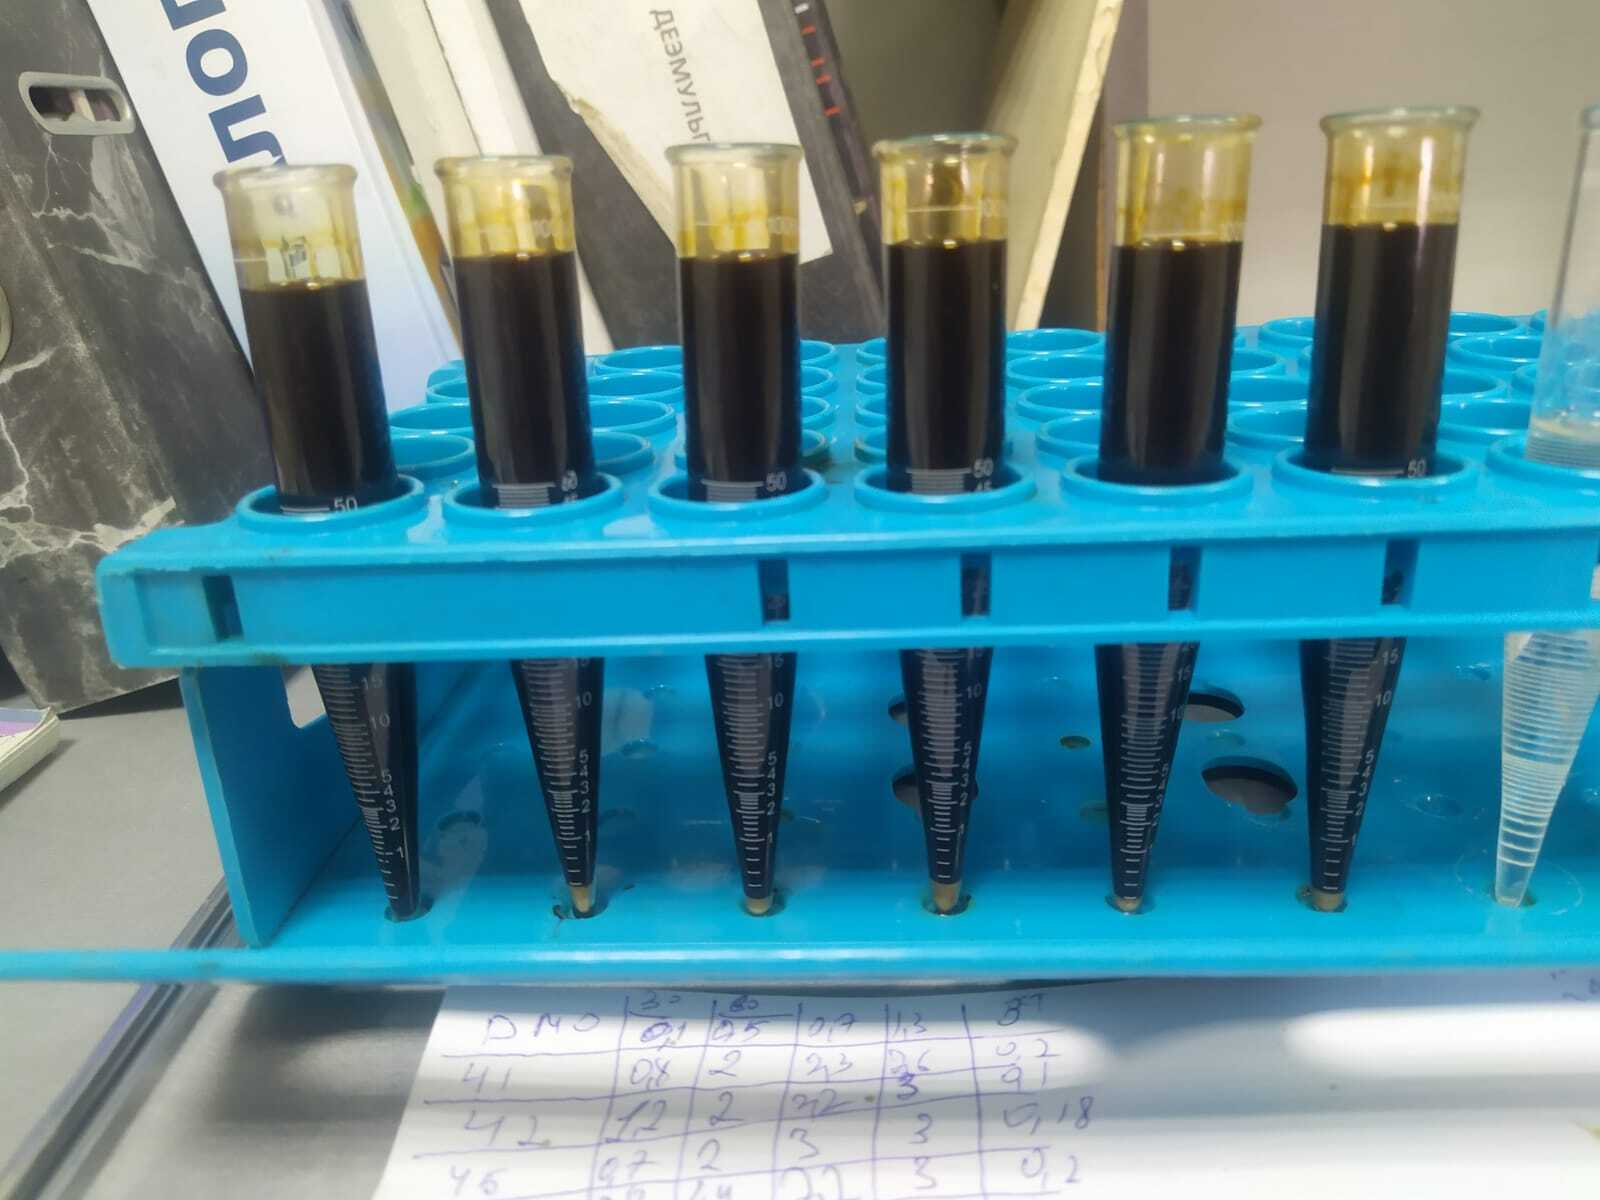
\includegraphics[width=0.8\textwidth]{assets/1075}
	\caption*{}
\end{figure}

{\bfseries Figure 1 - Oil samples after analysis}

After settling the emulsion by centrifugation, the residual water
content in the emulsion is determined.

No. 1 Analysis. MICH Test of Meerbusch30\% LLP + BNG 70\% LLP.

6 settling tanks with oil of m/r Kulzhan and Ayyrshagyl were installed
with the addition of a demulsifier in them in the equivalent of 70 grams
/ ton. Various models of the EASY-DE demulsifier were added to the tubes
and one tube was with a basic demulsifier labeled as "EASYDE 03-15".For
the reliability of the results, the analyses were carried out several
times.

No. 2 Analysis. MIX Meerbusch+BNG 50\% : 50\%

6 settling tanks with oil were installed m/r Kulzhan and Ayyrshagyl with
the addition of a demulsifier in them in the equivalent of 70 grams /
ton. Various models of the EASY-DE demulsifier were added to the tubes
and one tube was with a basic demulsifier labeled as "EASYDE 03-15".
Another test tube was left without the addition of reagents to compare
the work and determine the effectiveness of our reagents. For the
reliability of the results, the analyses were carried out several times.

No. 3 Analysis. MIX Meerbusch+BNG 30\% : 70\%

6 settling tanks with oil were installed m/r Kulzhan and Ayyrshagyl with
the addition of a demulsifier in them in the equivalent of 70 grams /
ton. Various models of the EASY-DE demulsifier were added to the tubes
and one tube was with a basic demulsifier labeled as "EASYDE 03-15".
Another test tube was left without the addition of reagents to compare
the work and determine the effectiveness of our reagents. For the
reliability of the results, the analyses were carried out several times.

{\bfseries Results and discussion.} The results of the tests on 6 samples
are shown in Tables 2-4.

{\bfseries Table 2 - Results of MICH Test of Meerbusch30\% LLP + BNG 70\%
LLP}

\begin{longtable}[]{@{}
  >{\raggedright\arraybackslash}p{(\columnwidth - 16\tabcolsep) * \real{0.1413}}
  >{\raggedright\arraybackslash}p{(\columnwidth - 16\tabcolsep) * \real{0.0950}}
  >{\raggedright\arraybackslash}p{(\columnwidth - 16\tabcolsep) * \real{0.0950}}
  >{\raggedright\arraybackslash}p{(\columnwidth - 16\tabcolsep) * \real{0.0950}}
  >{\raggedright\arraybackslash}p{(\columnwidth - 16\tabcolsep) * \real{0.0950}}
  >{\raggedright\arraybackslash}p{(\columnwidth - 16\tabcolsep) * \real{0.0950}}
  >{\raggedright\arraybackslash}p{(\columnwidth - 16\tabcolsep) * \real{0.1048}}
  >{\raggedright\arraybackslash}p{(\columnwidth - 16\tabcolsep) * \real{0.1286}}
  >{\raggedright\arraybackslash}p{(\columnwidth - 16\tabcolsep) * \real{0.1502}}@{}}
\toprule\noalign{}
\multirow{2}{*}{\begin{minipage}[b]{\linewidth}\raggedright
Reagent
\end{minipage}} & \multicolumn{6}{l}{%
\begin{minipage}[b]{\linewidth}\raggedright
Amount of separated water, ml
\end{minipage}} &
\multirow{2}{*}{\begin{minipage}[b]{\linewidth}\raggedright
Residual water ,\%
\end{minipage}} &
\multirow{2}{*}{\begin{minipage}[b]{\linewidth}\raggedright
Interfacial layer , \%
\end{minipage}} \\
& \begin{minipage}[b]{\linewidth}\raggedright
\emph{15} \emph{min}
\end{minipage} & \begin{minipage}[b]{\linewidth}\raggedright
\emph{30} \emph{min}
\end{minipage} & \begin{minipage}[b]{\linewidth}\raggedright
\emph{45} \emph{min}
\end{minipage} & \begin{minipage}[b]{\linewidth}\raggedright
\emph{60} \emph{min}
\end{minipage} & \begin{minipage}[b]{\linewidth}\raggedright
\emph{90} \emph{min}
\end{minipage} & \begin{minipage}[b]{\linewidth}\raggedright
\emph{120} \emph{min}
\end{minipage} \\
\midrule\noalign{}
\endhead
\bottomrule\noalign{}
\endlastfoot
ДНЭ-М & 0,1 & 0,1 & 0,3 & 0,5 & 0,7 & 1,3 & 0 & 0 \\
ED 03-15 & 0,1 & 0,1 & 0,1 & 0,1 & 0,1 & 0,2 & 0,2 & 0,15 \\
ED 03-41 & 0,4 & 0,8 & 1,6 & 2 & 2,3 & 2,6 & 0,2 & 0,16 \\
ED 03-42 & 0,7 & 1,2 & 1,6 & 2 & 2,2 & 3 & 0,1 & 0,1 \\
ED 02-45 & 0,3 & 0,7 & 1,4 & 2 & 3 & 3 & 0,18 & 0,1 \\
ED 01-46 & 0,4 & 1,4 & 1,8 & 2,2 & 2,8 & 3 & 0,2 & 0,2 \\
\end{longtable}

\emph{* ED -- EASY-DE}

\emph{Reagent dosage:70 g/ton}

\emph{Process temperature at the facility:55-500C}

\emph{Water content in oil:6\%}

{\bfseries Table-3. Results of MIX Meerbusch+BNG 70\% : 30\% analysis}

\begin{longtable}[]{@{}
  >{\raggedright\arraybackslash}p{(\columnwidth - 16\tabcolsep) * \real{0.1413}}
  >{\raggedright\arraybackslash}p{(\columnwidth - 16\tabcolsep) * \real{0.0950}}
  >{\raggedright\arraybackslash}p{(\columnwidth - 16\tabcolsep) * \real{0.0950}}
  >{\raggedright\arraybackslash}p{(\columnwidth - 16\tabcolsep) * \real{0.0950}}
  >{\raggedright\arraybackslash}p{(\columnwidth - 16\tabcolsep) * \real{0.0950}}
  >{\raggedright\arraybackslash}p{(\columnwidth - 16\tabcolsep) * \real{0.0950}}
  >{\raggedright\arraybackslash}p{(\columnwidth - 16\tabcolsep) * \real{0.1048}}
  >{\raggedright\arraybackslash}p{(\columnwidth - 16\tabcolsep) * \real{0.1286}}
  >{\raggedright\arraybackslash}p{(\columnwidth - 16\tabcolsep) * \real{0.1502}}@{}}
\toprule\noalign{}
\multirow{2}{*}{\begin{minipage}[b]{\linewidth}\raggedright
Reagent
\end{minipage}} & \multicolumn{6}{l}{%
\begin{minipage}[b]{\linewidth}\raggedright
Amount of separated water, ml
\end{minipage}} &
\multirow{2}{*}{\begin{minipage}[b]{\linewidth}\raggedright
Residual water ,\%
\end{minipage}} &
\multirow{2}{*}{\begin{minipage}[b]{\linewidth}\raggedright
Interfacial layer , \%
\end{minipage}} \\
& \begin{minipage}[b]{\linewidth}\raggedright
\emph{15 min}
\end{minipage} & \begin{minipage}[b]{\linewidth}\raggedright
\emph{30 min}
\end{minipage} & \begin{minipage}[b]{\linewidth}\raggedright
\emph{45 min}
\end{minipage} & \begin{minipage}[b]{\linewidth}\raggedright
\emph{60 min}
\end{minipage} & \begin{minipage}[b]{\linewidth}\raggedright
\emph{90 min}
\end{minipage} & \begin{minipage}[b]{\linewidth}\raggedright
\emph{120 min}
\end{minipage} \\
\midrule\noalign{}
\endhead
\bottomrule\noalign{}
\endlastfoot
Without reagent & 0,1 & 0,1 & 0,3 & 0,4 & 0,4 & 0,5 & 0,9 & 0 \\
ДНЭ-М & 0,1 & 0,1 & 2 & 4 & 4,4 & 5 & 0,1 & 0 \\
ED 03-15 & 0,4 & 2,5 & 2,6 & 2,8 & 3 & 3,5 & 0,1 & 0 \\
ED 03-40 & 0 & 0,15 & 0,5 & 1 & 1 & 1 & 0,2 & 0 \\
ED 02-14 & 0,3 & 2,5 & 3,8 & 5 & 6 & 6,5 & 0,4 & 0 \\
ED 01-09 & 0,4 & 1 & 3 & 5 & 5,3 & 6 & 0,2 & 0 \\
\end{longtable}

\emph{* ED -- EASY-DE}

\emph{Reagent dosage:75 g/ton}

\emph{Process temperature at the facility:55-500C}

\emph{Water content in oil:6\%}

{\bfseries Table-4 - Results of MIX Meerbusch+BNG 50\% : 50\% analysis}

\begin{longtable}[]{@{}
  >{\raggedright\arraybackslash}p{(\columnwidth - 16\tabcolsep) * \real{0.1413}}
  >{\raggedright\arraybackslash}p{(\columnwidth - 16\tabcolsep) * \real{0.0950}}
  >{\raggedright\arraybackslash}p{(\columnwidth - 16\tabcolsep) * \real{0.0950}}
  >{\raggedright\arraybackslash}p{(\columnwidth - 16\tabcolsep) * \real{0.0950}}
  >{\raggedright\arraybackslash}p{(\columnwidth - 16\tabcolsep) * \real{0.0950}}
  >{\raggedright\arraybackslash}p{(\columnwidth - 16\tabcolsep) * \real{0.0950}}
  >{\raggedright\arraybackslash}p{(\columnwidth - 16\tabcolsep) * \real{0.1048}}
  >{\raggedright\arraybackslash}p{(\columnwidth - 16\tabcolsep) * \real{0.1286}}
  >{\raggedright\arraybackslash}p{(\columnwidth - 16\tabcolsep) * \real{0.1502}}@{}}
\toprule\noalign{}
\multirow{2}{*}{\begin{minipage}[b]{\linewidth}\raggedright
Reagent
\end{minipage}} & \multicolumn{6}{l}{%
\begin{minipage}[b]{\linewidth}\raggedright
Amount of separated water, ml
\end{minipage}} &
\multirow{2}{*}{\begin{minipage}[b]{\linewidth}\raggedright
Residual water ,\%
\end{minipage}} &
\multirow{2}{*}{\begin{minipage}[b]{\linewidth}\raggedright
Interfacial layer , \%
\end{minipage}} \\
& \begin{minipage}[b]{\linewidth}\raggedright
\emph{15 min}
\end{minipage} & \begin{minipage}[b]{\linewidth}\raggedright
\emph{30 min}
\end{minipage} & \begin{minipage}[b]{\linewidth}\raggedright
\emph{45 min}
\end{minipage} & \begin{minipage}[b]{\linewidth}\raggedright
\emph{60 min}
\end{minipage} & \begin{minipage}[b]{\linewidth}\raggedright
\emph{90 min}
\end{minipage} & \begin{minipage}[b]{\linewidth}\raggedright
\emph{120 min}
\end{minipage} \\
\midrule\noalign{}
\endhead
\bottomrule\noalign{}
\endlastfoot
Without reagent & 0,1 & 0,2 & 0,2 & 0,2 & 0,2 & 0,2 & 0,9 & 0 \\
ДНЭ-М & 0,1 & 0,2 & 0,2 5 & 0,3 & 0,3 & 0,3 & 0,1 & 0 \\
ED 03-09 & 0,1 & 0,15 & 0,3 & 0,3 & 0,3 & 0,3 & 0,1 & 0 \\
ED 03-42 & 0 & 0,25 & 0,5 & 1 & 1,2 & 1,2 & 0,2 & 0 \\
ED 03-15 & 0,1 & 0,2 & 0,3 & 0,4 & 0,4 & 0,4 & 0,4 & 0 \\
ED 01-10 & 0,4 & 0,9 & 3 & 3,5 & 3,5 & 4,5 & 0,2 & 0 \\
\end{longtable}

According to the results of analyzes of oils in different ratios,
demulsifiers DE 03-15, DE 03-42, as well as DNE-M showed good results in
separating water from crude oil.

Reagent DE 03-15 works effectively with a crude oil in a ratio of 70:30
(Meerbusch: BNG), as well as 50:50 (Meerbusch: BNG), when oil with a
significant content of mechanical impurities and chloride salts is mixed
with oil, which contains relatively more paraffins .

At a ratio of 30:70 (Meerbusch: BNG), where oil with a high paraffin
content predominates, the effectiveness of the demulsifier decreases. In
this case, the DE 03-42 reagent is more effective.

Demulsifier 03-15 is more preferable for the preparation of these oils
in a 50:50 ratio, since the economic cost of this reagent is
significantly lower compared to analogues, and the phase boundary
between the oil and water layers is thinner.

A comparative analysis of the research results showed that at a settling
temperature of +55° With the most effective demulsifier for the
preparation of water-oil emulsions, the Meerbusch LLP+ BNG LLP is
EASY-DE03-15.

The dynamics of water release from water-oil emulsions in the free phase
exceeds the indicators of tested demulsifiers. Residual content of water
and undisturbed emulsion in the settled oil: the demulsifier of the
EASY-DE03-15 brand is superior to other reagents showing a smaller
amount of water and undisturbed phase. The quality of the oil-water
phase section: the intermediate layer in the settling tanks is not
noticed.

The released water has no turbidity, transparent without noticeable
traces of oil.

The content of chloride salts in oil has decreased by 3 times due to the
fact that the inorganic chloride salts, which are dissolved in the
aqueous phase, separated along with water.

As a result of the conducted research, it can be concluded that the
resulting composition in the oil processing in field conditions reduces
the influence of aggressive media on the metal surface, as well as
reduces the formation of salt deposits and prolongs the formation time
of deposits. Because of this, various salt deposits contained in oil
allow it to settle in tanks with raw materials. When preparing oil for
processing, reducing the content of reservoir water and salts prevents
the formation of deposits on the surface of the equipment.

It has been established that the EASY-DE 03-15 demulsifier is the most
effective reagent for dehydration of oil-water emulsions and
desalination of MIX samples of Meerbusch LLP + BNG LLP. The demulsifier
EASY-DE 03-15 works perfectly with medium-density oil that contains
various natural impurities, such as chloride salts, mechanical
impurities, and paraffins. The relatively average density of oils also
indicates that they might also contain asphaltenes in a certain amount,
which also stabilize the oil-water emulsion.

{\bfseries Conclusion.} Thus, the results of research reveal that
Demulsifier EASY-DE03-15 is recommended for conducting pilot industrial
testing to obtain the final result of applicability at the facilities of
dewatering and desalination of oil samples of Meerbusch LLP + BNG LLP
except for the treatment of oil with fresh water.

Analyzing the stability of oil emulsions depending on the washing water,
according to the demulsifier flow rates that ensure its separation, it
was found that the effectiveness of the demulsification process is
influenced by the interaction of two factors: the aqueous phase and the
degree of its dispersion. Since the process of demulsification of oil
using a demulsifying reagent is associated with the destruction and
adsorption displacement of natural stabilizers at the oil-water boundary
by demulsifying molecules, an increase in water content has a strong
effect on the consumption of oil by the reagent.

Thus, the results of the conducted experimental studies show that with
an increase in the water saturation of oil, the consumption of the
demulsifier decreases. At the same time, by purposefully increasing the
water saturation of the finished rheologically complex oil to its
maximum value, it is possible to reduce the consumption of the
demulsifier several times without reducing the efficiency of the oil
dewatering process. In this connection, it can be stated that the
effectiveness of using demulsifiers of domestic production was proved.
Use of domestic demulsifier has certain advantages over imported ones
{[}14{]}.

{\bfseries References}

1.Godzhaev E.M., Mamedov Je.A., Musaev T.P., Alieva Ash. Vybor i
issledovanie himicheskih reagentov dlja poluchenija
dejemul\textquotesingle gatorov. //Aktual\textquotesingle nye problemy
gumanitarnyh i estestvennyh nauk Nauchnoe izdatel\textquotesingle stvo
"Institut strategicheskih issledovanij,2018.-№ 1(2) - S.5-8.{[}in
Russ.{]}

2. Gladij E.A., Kemalov A.F., Gajnullin V.I Ocenka jeffektivnosti
shiroko primenjaemyh reagentov-dejemul\textquotesingle gatorov dlja
obezvozhivanija nefti termohimicheskim sposobom // Jekspozicija
Neft\textquotesingle{} Gaz.-2015.- № 5 (44).- S.18-20. {[}in Russ.{]}

3.Ochilov A.A.Razrushenie ustojchivyh vodoneftjanyh
jemul\textquotesingle sij mestnyh neftej
dejemul\textquotesingle gatorami serii D// Molodoj
uchenyj,2015.-T.8(88)- S.283-286. {[}in Russ.{]}

4.Nurlybaj S.A., Buzova O.V. Issledovanie vlijanija razlichnyh faktorov
na stabil\textquotesingle nost\textquotesingle{} vodoneftjanoj
jemul\textquotesingle sii // Vestnik Kazahstansko-Britanskogo
tehnicheskogo universiteta, 2019.- T.16(4)- S.9-18. {[}in Russ.{]}

5. Geritz B. Methods of destruction of crude oil emulsion.// Oil
industry.- 2018.- Vol.3(10)- P.89-94.

6.Bashkirceva N.Ju., Sladovskaja O.Ju., Rahmatullin R.R., Mingazov R.R.,
Ganieva T.F. Primenenie poverhnostno-aktivnyh veshhestv v processah
podgotovki i transportirovki nefti -- //Kazan\textquotesingle:
KNITU.-2016.-S.168-172.{[}in Russ.{]}

7.Sadyrbaeva A.S., Bajbotaeva S.E., Turebekova A.M., Zhanabaj S.Zh.
Jeffektivnost\textquotesingle{} vozdejstvija
dejemul\textquotesingle gatora na process razrushenija vodoneftjanyh
jemul\textquotesingle sij // Mezhdunarodnyj studencheskij nauchnyj
vestnik -2019. - № 2 -- S.56-64. {[}in Russ.{]}

8. Serkebaeva B.S., Myrzagalieva K.N. Optimizacija tehnologii
primenenija dejemul\textquotesingle gatorov // Neft\textquotesingle{} i
gaz: sb. tez. -M.- 2015. -T.1. -- 391s. {[}in Russ.{]}

9. Ahmetov S.A. Lekcii po tehnologii glubokoj pererabotki nefti v
motornye topliva.//Sankt-Peterburg: Nedra.- 2007. -312 s. {[}in Russ.{]}

10. Al-Sabagh AM, Noor El-Din MR, Kandile N. Functions of Demulsifiers
in the Petroleum Industry. //Separation Science and Technology.- 2011.-
Vol.46(7).- P.1144-1163.

DOI:10.1080/01496395.2010.550595

11. Sattorov M.O., Jamaletdinova A.A., Bakieva Sh.K. Analiz
jeffektivnosti dejemul\textquotesingle gatorov, primenjaemyh pri
razrushenie mestnyh vodoneftjanyh jemul\textquotesingle sij //
Universum: tehnicheskie nauki.- 2020.- № 4. - S. 73-76. {[}in Russ.{]}

12.Sattorov M.O. Opredelenie sostava komponentov
polimerov-dejemul\textquotesingle gatorov razlozhenija vodoneftjanyh
jemul\textquotesingle sij. Mezhdunarodnyj nauchno-prakticheskij zhurnal
``Teorija i praktika sovremennoj nauki''. 03(45), 2019 g.S.260-262.
{[}in Russ.{]}

13. Trushkova L.V. Metodiki ocenki jeffektivnosti reagentov
dejemul\textquotesingle gatorov / L.V. Trushkova, Ju.A. Sarycheva /
Neft\textquotesingle{} i gaz zapadnoj Sibiri:Materialy
nauchno-prakticheskoj konferencij -- Tjumen\textquotesingle:Tjumenskij
industrial\textquotesingle nyj universitet- 2015.- P.210--213. {[}in
Russ.{]}

14. Ismajylov G.G., Izbasarov E.I., Adygezalova M.B., Halilov R.Z..
Issledovanie vlijanija reagentov-dejemul\textquotesingle gatorov na
kinetiku obezvozhivanija reologicheski slozhnoj nefti//Vestnik PNIPU.
Geologija. Neftegazovoe i gornoe delo.- 2017.- T.16 (2). - S.138 - 147.
{[}in Russ.{]}

\emph{{\bfseries Information about the authors}}

Tastanova Lyazzat. Knashevna -- Candidate of Chemical Sciences,
Associate Professor, Aktobe Regional university named after K.Zhubanov,
Aktobe, Kazakhstan, е-mail: lyazzatt@mail.ru;

Apendina Ainagul Kenesovna - Candidate of Chemical Sciences, Aktobe
Regional university named after K.Zhubanov, Aktobe, Kazakhstan, е-mail:
K.Ajnagul@mail.ru;

Orynbasar Raigul Orynbasarovna - Candidate of Chemical Sciences, docent,
Aktobe Regional university named after K.Zhubanov, Aktobe, Kazakhstan,
е-mail: raihan\_06\_79@mail.ru;

Zhanserikov Nurmukhammed Zhanserikuly - Master of Science, Chemical
analysis laboratory assistant, IC Petroleum, Aktobe, Kazakhstan, е-mail:
zanserikovnurmuhammed@gmail.com;

Nurlybay Sultan Alimzhanuly - Master of Science, University teacher,
Aktobe Regional university named after K.Zhubanov, Aktobe, Kazakhstan,
ORCID 0009-0001-8466-8539, Казахстан, е-mail: su1tan@bk.ru

\emph{{\bfseries Сведения об авторах}}

Тастанова Л.К. -к.х.н., ассоциированный профессор, Актюбинский
Региональный университет им. К. Жубанова, Актобе, Казахстан, е-mail:
lyazzatt@mail.ru;

Апендина А.К. - к.х.н., Актюбинский Региональный университет им.
К.Жубанова, Актобе, Казахстан, е-mail: K.Ajnagul@mail.ru;

Орынбасар Р.О.- к.х.н., доцент, Актобе, Казахстан, к.х.н., Актюбинский
Региональный университет им. К.Жубанова, е-mail: raihan\_06\_79@mail.ru;

Жансериков Н.Ж.-магистр, IC Petroleum, Актобе, Казахстан, е-mail:
zanserikovnurmuhammed@gmail.com;

Нұрлыбай С. Ә.-магистр, преподаватель, Актюбинский Региональный
университет им. К.Жубанова,Актобе, Казахстан, e-mail:su1tan@bk.ru
